\documentclass{paper}
\usepackage{times}
\usepackage{geometry}
\geometry{letterpaper, portrait, margin=1in}
\usepackage{setspace} \doublespacing
%\usepackage{setspace} \singlespacing
\usepackage[utf8]{inputenc}
\usepackage{enumitem,amssymb}
\usepackage{ragged2e}
\usepackage{physics}
\usepackage{siunitx}
\usepackage{wasysym}
\sisetup{separate-uncertainty=true}
\usepackage{float}
\usepackage{mathtools}
\usepackage{amsmath}

\usepackage{caption}
\usepackage[hidelinks]{hyperref}
\usepackage{url}

\usepackage{graphicx}
\usepackage{epstopdf}
\usepackage{tikz}
\graphicspath{{data/concepts}}

\usepackage{aas_macros}
\usepackage[style=authoryear]{biblatex}
\bibliography{refs} %refs.bib
\nocite{*}

\immediate\write18{texcount \jobname.tex -out=\jobname.sum}

% set frameboxes to be borderless
\setlength{\fboxsep}{0pt}
\setlength{\fboxrule}{0pt}

\begin{document} 

\title{The constituents of the universe and the growth of structure}
\author{ariahayd}
\date{April 24, 2022}
\maketitle

% Overview. [8]
% Give an overview of the current standard model for the context of the essay. 
% Include one figure for this section. 
\section*{Overview}
  The universe is shaped by its constituent energies, and its constituents are
  shaped by the size of space. The evolution of the universe is understood 
  through the Standard Model of Cosmology, developed over the last 
  century of observations of matter and energy on large scales, of structures 
  in cubic gigaparsec volumes space, and on small scales 
  where the quantum mechanical properties of energy fields emerge. 

  The most successful model is $\Lambda$CDM, the concordance model, with 
  dynamics explained through General Relativity and Quantum Field Theory, 
  with contributions from dark energy ($\Lambda$) and cold dark matter 
  (CDM). These last two components are observationally confirmed but not 
  entirely explained by theory. 

  The densities of energy in the fields within the Universe determine the 
  geometry of space.  Observations indicate that the curvature of the metric 
  of spacetime over large distances is nearly flat and has been throughout 
  most of the history of the universe.
  
  $\Lambda$CDM is based on a Hot Big Bang (HBB) origin of high energy density 
  that has since evolved to today's universe of lower density. 
  Principal evidence of a HBB is from a homogeneous distribution of 
  quasar radio signals observed isotropically throughout space, but all 
  distant in time, indicating that the environments of galaxies were very 
  different in the past (\cite{Secrest_2021}) and that the universe is not in 
  an eternal steady state. 

%  The standard model explains how energy fields latent in space express in 
%  different ways in different evolutionary epochs, expanding the scale of 
%  space in the inflationary and current epochs, and smoothing out the 
%  distribution of gravitationally bound particles in the radiation dominated 
%  era. An illustration of this timeline is shown in Fig. 
%  \ref{fig:Intro-big_bang}. 
% The main successes of $\Lambda$CDM are 
% explanations of the origin of the abundances of observable matter and 
% primordial photons in the universe that come from these fields.

% \begin{figure}[H]
%   \begin{centering}
%   \includegraphics[scale=0.8]{Intro-big_bang.pdf}
%   \caption{A timeline of the hot big bang with times for each epoch,
%     along with the average temperature, and average energy per particle.
%   Credit: \cite{2016Ling}}
%   \label{fig:Intro-big_bang}
%   \end{centering}
% \end{figure}

   The standard model explains how energy fields latent in space express in 
   different ways across evolutionary epochs, expanding the scale of 
   space in the inflationary and current epochs, and smoothing out the 
   distribution of gravitationally bound particles in the radiation dominated 
   era. The main success of $\Lambda$CDM is the accounting of the energies
   that come from these fields, as shown in Fig. \ref{fig:Intro-constraints}. 

  \begin{figure}[H]
    \begin{centering}
    \includegraphics[scale=0.7]{Intro-constraints.pdf}
    \caption{The Sloan Digitial Sky Survey updated data release, including 
      measurements of the cosmic microwave background (CMB) from the Planck,
      mission places constraints on the parameters of $\Lambda$CDM, including
      energy from pressureless CDM, photons, baryons, neutrinos, and dark
      energy.
    Credit: \cite{2021PhRvD.103h3533A}}
    \label{fig:Intro-constraints}
    \end{centering}
  \end{figure}

% A hot big bang can be derived from an analysis of the metric of spacetime 
% applied to a homogeneous universe combined with observations of the 
% isotropic recession of luminous objects. The assumption that the total 
% volume of the universe holds a finite energy implies a positive curvature to 
% space and an eventual collapse under self-gravitation. That the collapse has 
% not happened, and to force a long term steady-state to the geometry of the 
% universe, led the original authors to include a $\Lambda$ term in the 
% cosmology (\cite{10.1093/mnras/90.7.668}). The standard model today is based 
% on the same terms, but explains the detail through different physics on
% small and large scales, on the scale of particles to galaxies clusters.

% 2. Dark Matter. [20]
% Describe two lines of evidence for dark matter. These should be distinct and 
% complementary. A line of evidence can consist of more than one observational 
% phenomenon that together provide the evidence. Include two figures for this 
% section.
\section*{Dark Matter}
  Large, gravitationally bound systems such as galaxies and galaxy clusters 
  appear embedded in gravitational potentials deeper than expected given 
  the masses observed interacting within the system. The depth of these 
  potentials is inferred due to unseen, \textit{dark} matter.

  % line of evidence one
  Early evidence for dark Matter in the halo of a galaxy comes from
  measurements of the rotational velocities of the material in the arms of
  spiral galaxies. A spiral galaxy is a stable, virialized structure bound by
  gravity and is expected to follow the Newtonian gravitation model for a
  fluid rotating around a center mass. The spiral arms are not coherent
  structures in themselves, but are the result of a density way propagating 
  through the fluid of the galactic disk. 

  The rotational velocity of the disk can be estimated via the 
  width of the HII emission lines across the disk of the galaxy, as was done
  for M31 (\cite{1970ApJ...159..379R}), showing the velocity field follows a 
  profile more like a rotating solid body a fluid 
  swirling around a core. Because galaxies can indeed be modeled 
  hydrodynamically, the only explanation for a velocity field continuing 
  beyond the visible matter of the galaxy is for an unobservable mass 
  encircling the galaxy in a halo.

  \begin{figure}[H]
    \begin{centering}
    \includegraphics[scale=0.4]{DM-masscurve.pdf}
    \caption{Fourteen different mass models fitting the velocity map data of
      M31 are combined to yield a band of mass estimates, on the left, and 
      surface densities, on the right, from the center to beyond the luminous 
      edge of M31, a galaxy with an has an apparent angular diameter of 
      \SI{178}{arc-minutes}.
    Credit: \cite{1970ApJ...159..379R}}
    \label{fig:DM-masscurve}
    \end{centering}
  \end{figure}

  The projected mass sheets of these halos are responsible for strong and weak 
  gravitational lensing. Since these early observations, dark matter halos 
  have been measured for most bound systems on the scale of galaxies or 
  clusters, though there is also evidence of anomalous galaxies that may lack 
  a significant concentration of dark matter around them 
  (\cite{10.1093/mnras/stab3491}). 

  Halos have been demonstrated to move with core material of galaxies and not 
  with energetic plasma that makes up majority of baryonic mass in a galaxy when 
  the plasma is disrupted by ram-pressure stripping. 
  Dark matter is bound to the gravitational potential of the galaxy rather 
  than to the baryons in the potential (\cite{Clowe_2006}). This observation 
  reinforces the \textit{cold} nature of dark matter; it cannot kinetically 
  escape the potential that binds baryonic masses, indicating that it 
  is decoupled from interactions with baryons. 

  %line of evidence two
  That dark matter could not be constituted entirely from baryonic particles
  follows from 
  solutions to the HBB model of the radiation era that show 
  pressure waves traveling through the irradiated plasma damping the
  accretion of the baryonic matter in any potential wells evident in the 
  anisotropy of spherical harmonic modes in the CMB.

  The baryon acoustic oscillation (BAO) signal comes from modeling the destructive
  interference pattern of the coupled photon-baryon fluid that permeated the
  radiation-dominated era of the Universe. The restoring force of a pressure
  variance in this fluid comes from the ionization and scattering between
  primordial atoms and photons interacting frequently due to the overwhelming
  prevalence of high energy photons resulting from baryogenesis, when most 
  baryons annihilated with their anti-particle pair, converting to photons.

  Gravitational fluctuations must have been built prior to the decoupling and 
  could not have been solely due to density variations in the photon-baryon 
  fluid.  There must have been a dark matter component to the ``frozen'' into 
  the environment of the plasma, seeding the gravitational fluctuations that 
  would quickly accrete material after decoupling, forming galaxies.
  As shown in Fig. \ref{fig:DM-BAO}, the number 
  density of galaxies in volumes of space, measured through redshift surveys, 
  correlates to the BAO signal at the scale of an earlier period in the 
  Universe.

  % \cite{2007MNRAS.381.1053P}
  
  % How small were the first cosmological objects?
  %The minimum baryonic mass that can become virialized is a function of \(z\),
  %from \SI{E6}{\astrosun} at \(z=15\) 
  % \cite{1997ApJ...474....1T}

  Explanations of dark matter can be categorized two ways; either due to 
  massive, compact halo objects (MACHOs) or by weakly interacting massive 
  particles (WIMPs). Searches for the lensing events from MACHOs in a galactic 
  halo have returned no significant findings. Though dark matter can be 
  observed through phenomena understood in the standard model, there is 
  no identified candidate WIMP particle that could constitute dark matter. An 
  explanation of the WIMP contribution to dark matter from something like a 
  primordial, massive graviton, requires new physics 
  (\cite{PhysRevLett.128.081806}).

  \begin{figure}[H]
    \begin{centering}
    \includegraphics[scale=0.5]{DM-BAO.pdf}
    \caption{A combination of two galaxy surveys shows the correlation of
      the density of galaxies with modeled density distribution from the
      BAO wave modes in the coupled photon-baryon
      fluid of the radiation dominated era. $k$ is the wave number of 
      an oscillating pressure wave. \(h = 0.7\) is the dimensionless Hubble
      constant. These observations match a model with a total energy density
      due to matter, \(\Omega_m = 0.25\), while the baryonic contribution is
      observed to be \(\Omega_b = 0.05\), indicating that the 
      difference is dark matter (\cite{Eisenstein_2005}).
    Credit: \cite{2007MNRAS.381.1053P}}
    \label{fig:DM-BAO}
    \end{centering}
  \end{figure}

% 3. Baryons. [20]
% Describe one indirect constraint on the baryon density (BBN or CMB), and key 
% direct measurements of various baryonic components. Include two figures for 
% this section.
\section*{Baryons}
  Constraints on the density of baryons among the energies of the universe are
  based on modeling the prevalence of atoms generated during the big bang 
  nucleosynthesis (BBN) epoch or by modeling angular size of spherical harmonic 
  patterns in the surface of last scattering of decoupling. Both 
  approaches for constraining the baryonic contribution to the matter density 
  are indirect because the methodologies infer the baryonic prevalence from 
  understood physics at early times rather than from direct measurements.

% That primordial chemical elements would have been produced in the 
% environment of a hot big bang, and that the duration of expansion rather 
% than temperature would determine the prevalence of elements, was theorized 
% (\cite{PhysRev.73.803}) before the term ``big bang'' was coined 
% (\cite{Hoyle1949}) and well before the debate over a big bang or continuous 
% creation origin had been decided.

  Particles coalesced in at least four distinct epochs. The end of the first era,
  the X-boson Era, at \SI{E-38}{s}, fixed the baryon and lepton number. 
  In the second, the Quark-Hadron Era, quarks combined to form baryonic 
  nucleons. This era ends at \SI{E-6}{s} with an asymmetry between baryonic
  particle and antiparticle pairs, in which normal baryons are estimated with an 
  excess of \SI{E-9} per pair (\cite{1993PhRvL..70.2833F}). The third, the 
  Lepton Era, ends at \SI{1}{s} as the temperature decreases to 
  where neutrinos are no longer coupled to electron-positron pairs, and can 
  escape reactions. Throughout these eras, WIMPs are expected to have been 
  present in the background contributing to local density fluctuations 
  through gravitation, but not through interactions.

  The fourth epoch, the Nucleosynthesis Era, between \SI{1}{s} and 
  \SI{300}{s}, was the duration over which weak force interactions changed
  the frequency distribution of protons and neutrons and primordial atomic 
  nuclides formed. The prevalence of free neutrons was constrained by both
  processes, and the resulting abundances of light elements throughout the 
  Universe generally matches the Standard BBN (SBBN)
  prediction. SBBN is based on the foundational physics of $\Lambda$CDM 
  during the radiation dominated era and the inclusion of three neutrino 
  species (\cite{Cyburt_2016}). 

  Weak interactions maintained the balance of protons and neutrons early in
  the Nucleosynthesis Era until the declining temperature of the fluid reduced 
  the likelihood of producing the neutron, slightly heavier than the proton, 
  within the reaction balance. At \(T = \SI{E10}{K}\), the fraction of 
  neutrons to all baryons froze at \(18\%\). This represents the neutron 
  budget for further nuclear reactions that produce primordial atomic nuclei, a budget
  declining exponentially over the next \SI{886}{s} following the 
  characteristic timescale for the decay of free neutrons through \(\beta\)
  emission.

  Atomic nuclei do not grow through many-body reactions 
  because the cross section of interaction for several specific particle
  ingredients needed to form a nucleus is rare. Instead, nuclei are built
  through a chain of two-body reactions. The first reaction in the chain
  combines a proton with a neutron to form deuterium. However, a deuterium
  nucleus is not tightly bound and can easily be broken back into constituent
  particles by interactions with photons until temperature of
  \(T = \SI{E9}{K}\), which happened at \(t = \SI{300}{s}\). After this point in cooling, 
  deuterium nuclei were available to form \(\prescript{3}{}{He}\), 
  \(\prescript{4}{}{He}\), \(\prescript{6}{}{Li}\), \(\prescript{7}{}{Li}\), 
  and \(\prescript{7}{}{Be}\) through chains that reach equilibrium on
  timescales shown in Fig. \ref{fig:BBN-frac}.

  \begin{figure}[H]
    \begin{centering}
    \includegraphics[scale=0.3]{BBN-frac.pdf}
    \caption{A chart of the mass fraction of baryons and nuclides over the
      SBBN era. Note that the fraction of protons remains essentially static
      while neutrons are consumed to make nuclides. The mass fraction of 
      neutrons declines overall, but drops precipitously after 
      \(t = \SI{200}{s}\) as the neutron number fraction among baryons froze 
      and the characteristic lifetime of unbound neutrons allowed rapid decay.
      The mass fractions of primordial nuclides heavier than 
      \(\prescript{4}{}{He}\) are vanishingly small.
    Credit: \cite{ryden2003introduction}}
    \label{fig:BBN-frac}
    \end{centering}
  \end{figure}

  Measuring the metal content of stars in the least active globular clusters, 
  which are presumed to be the best preserved early environments that can be 
  observed nearby, approximates but does not exactly match the predicted 
  abundances of SBBN atoms. This indicates some stellar processing prior to 
  the oldest clusters \cite{Kalirai_2010}. Using clusters as ``chronometers'' 
  suggests a time since the HBB of 
  \SI{15.6(46)E9}{years} (\cite{1999ApJ...521..194C}).
  Fig. \ref{fig:BBN-ratios} shows the observed abundances within predicted
  ranges.

  %baryongensis is a process that violates CP conservation
  %In the standard model of cosmology, baryon number is not conserved
  %(\cite{PhysRevLett.37.8}). From the
  %(\cite{DINE1991351})

  Most of the baryons in the universe, 75\%, are not gravitationally bound in 
  structures like galaxies, but are diffuse in the intergalactic medium. By 
  measuring the dispersion, the delay in repeated signaling of fast radio 
  bursts through a modeled column of electrons relative to a true vacuum with 
  no particles to scatter the photons, the unbound baryonic matter has been 
  measured at \(\Omega_b = 0.051\) (\cite{2020Natur.581..391M}).

  \begin{figure}[H]
    \begin{centering}
    \includegraphics[scale=0.4]{BBN-ratios.pdf}
    \caption{A modeled prediction of the abundances of nuclides through big
      bang nucleosynthesis assuming a neutron characteristic lifetime of
      \(\tau_n = \SI{880.3(11)}{s}\) and a neutrino species number of 3. 
      \(Y\) is the fraction of primordial \(\prescript{4}{}{He}\). The width 
      of each band is related to the uncertainty in the cross-section of 
      interaction for each nuclear species. Boxes in the figure are values 
      allowed by observations. The vertical striped band is the constraint 
      based on observations of deuterium, limiting 
      \(0.043 \leq \Omega_b \leq 0.051\), while the crosshatched band 
      is the inference of \(\Omega_b\) from the CMB. Note that values for 
      \(\prescript{7}{}{Li}\) do not match observation. The baryon to photon 
      ratio is a range of excess photons resulting from baryon pair 
      production.
    Credit: \cite{liddle2015introduction}}
    \label{fig:BBN-ratios}
    \end{centering}
  \end{figure}

  %Correlation function galaxy distribution as constraint on DE
  % \cite{2003ApJ...594..665B}

% 4. Dark Energy. [20]
% Describe two lines of evidence for dark energy. Comment on possible 
% modifications to the standard model. Include two figures for this section.
\section*{Dark Energy}
  The energy density of the Universe seems to drive towards
  a flat spatial metric even at points in the
  the standard model evolution of the universe which could be expected
  to deviate from the critical density due to the shaping effects of 
  energy densities.

  The pressure nudging spacetime to a flat curvature in the current epoch is 
  known as \textit{dark} energy, the $\Lambda$ component of the $\Lambda$CDM
  model, because the source of energy has not yet been explained. 
  It is thought to be a constant, latent energy density of the vacuum of 
  spacetime in a phase above a potential ground state.

  Evidence for dark energy in the $\Lambda$CDM model comes from two 
  significant observations that independently constrain the contribution of 
  $\Lambda$ to the energy budget, namely measurements of the recession of 
  supernovae as standard candles, shown in Fig. \ref{DE-sn_lightcurve}, and 
  measurements of the angular size of 
  standard rulers in the CMB anisotropy, in Fig. \ref{DE-MCMC}.

  Assuming redshift to be a proxy for
  distance, the Hubble diagram in Fig. \ref{fig:DE-sn_lightcurve} shows an 
  increase in recession 
  velocity with distance, implying an acceleration between
  the positions of observation and event against the rest frame of a
  fundamental observer. The Supernova Cosmology Project later
  added ten more supernova events to this diagram 
  (\cite{2012ApJ...746...85S}).

  % supernovae \cite{Riess_1998}
  \begin{figure}[H]
    \begin{centering}
    \includegraphics[scale=0.4]{DE-sn_lightcurve.pdf}
    \caption{The figure on the top is a fit of measurements of the multicolor 
      light curve shape (MLCS) characteristic of SNe Ia as a function of 
      measured redshift of the event spectrum. The figure below is the
      difference between measured magnitude and modeled magnitude for an 
      environment with no dark energy to show that observations convincingly 
      deviate from an \(\Omega_{\Lambda} = 0\) 
      environment.
      Credit: \cite{Riess_1998}}
    \label{fig:DE-sn_lightcurve}
    \end{centering}
  \end{figure}

% \begin{figure}[H]
%   \begin{centering}
%   \includegraphics[scale=0.6]{DE-constraints.pdf}
%   \caption{Constraints on the free parameters of the $\Lambda$CDM
%     model predicting a range of values for \(\Omega_{m}\) and 
%     \(\Omega_{\Lambda}\). The topographic lines of each parameter represent 
%     confidence intervals in the measurement. This figure excludes systematic
%     errors in the supernovae measurements.
%     Credit: \cite{2012ApJ...746...85S}}
%   \label{fig:DE-constraints}
%   \end{centering}
% \end{figure}

  \begin{figure}[H]
    \begin{centering}
    \includegraphics[scale=0.5]{DE-MCMC.pdf}
    \caption{Constraints on the free parameters of the $\Lambda$CDM
      model predicting a range of values for \(\Omega_{\Lambda}\). The contour 
      lines of each parameter represent confidence intervals in the 
      measurement. The values for \(\Omega_{\Lambda}\) are projected from
      Markov chain Monte Carlo (MCMC) simulations of inputs from Wilkinson 
      Microwave Anisotropy Probe (WMAP) data across the parameter space 
      (\cite{Bennett_2011}). For inputs in the domain of likely values for 
      \(\Omega_b\) and \(\Omega_c\) (CDM), the models independently agree at 
      \(\Omega_{\Lambda} \approx 0.73\).
    Credit: \cite{liddle2015introduction}}
    \label{fig:DE-MCMC}
    \end{centering}
  \end{figure}

  Alternatives to the $\Lambda$CDM model include
  modifications to the equation of state for dark energy, assumed to have a
  constant value of \(w = \frac{P}{\rho c^2} = -1\) for the modern epoch. 
  Instead, the energy density is fixed
  to the grid of spacetime and expressed as a pressure on volumes of
  vacuum that becomes more significant where the matter density drops, as it
  has in the current epoch, to \(w = -\frac{1}{3}\). This model is 
  called \textit{quintessence}, is considered to be distinct from a 
  cosmological constant, but with a similar effect on observations
  (\cite{PhysRevLett.80.1582}). 

  In this modification to $\Lambda$CDM the source of pressure from dark 
  energy is a latent scalar field coupled to the geometry of the universe, 
  resulting in spacetime growth under an \(R_h = ct\) model, and may currently 
  fit observations best when compared across models and input parameters 
  (\cite{10.1093/mnras/sty1962}).

% 5. Growth of structure. [24]
% Describe how initial fluctuations from inflation have grown to form galaxies. 
% Consider the growth rate on various scales, and the different behaviour of 
% dark matter and baryons.  Include two figures for this section. 
\section*{Growth of Structure}

  Galaxies and galaxy clusters are the largest gravitationally
  bound structures directly observed. Because a galaxy is a bound object,
  it may be assumed to have not changed size with cosmological inflation,
  so would have the same size today as when it stabilized. 
  The era that separated one galaxy from the 
  constant background density of the universe occurred at redshift of 100.
  The model for collapse of the background density into a bound, virialized
  structure is the Jeans criteria and is highly dependent on the thermal 
  velocity and mass density of a fluid (\cite{Jeans1902}).

  \begin{figure}[H]
    \begin{centering}
    \includegraphics[scale=0.5]{Struct-mass.pdf}
    \caption{A graph of the minimum mass needed to collapse into a virialized
      structure over time. Masses in 
      the light, unshaded region can collapse and become luminous. 
      The dashed lines represent 
      constant post-virialization temperatures of \SI{E4}{K} and \SI{E3}{K}. 
      The darkest shaded region cannot cool through radiative means because 
      the temperature after virializing would be the same as the cosmic 
      microwave background. The solid line is drawn to show about where 
      \(\Omega_b \times \SI{2E6}{M_{\astrosun}}\) can collapse at \(z=30\).
    Credit: \cite{1997ApJ...474....1T}}
    \label{fig:Struct-mass}
    \end{centering}
  \end{figure}

  The minimum mass for gravitational collapse after the radiation dominated
  era, with an initial temperature of \(T \approx \SI{3000}{K}\), is on the 
  order of \SI{E5}{M_{\astrosun}}, shown in Fig. \ref{fig:Struct-mass}.
  This is lower than the masses of galaxies and about 
  similar to the mass of globular clusters.
  The Jeans criteria indicates that galactic masses could certainly have 
  coalesced into virialized structures in the time since decoupling.

  The photon-baryon fluid plasma of the early universe was concurrent with a field of 
  dark matter particles that, through fluctuations in its density 
  distribution, created the initial seeds for structural growth. The plasma 
  was not coupled to the dark matter other than through gravitation, causing
  a feedback loop in the evolution of the fields. A smoothness in the density
  of the plasma was enforced through electromagnetic interactions between the ions and
  photons. 
  This smoothness prevented the plasma from 
  accreting into the gravitational potentials of the dark matter. In turn, the 
  dark matter could not further collapse into the potential wells due 
  to pressure from the fluid, the Silk damping effect.  

  Two thermodynamic models explain how the plasma 
  would have evolved through the radiation-dominated era. Hierarchical
  formation assumes an adiabatic fluid that formed large scale structure 
  before splitting into smaller scale structures. Bottom-up formation
  begins with structures on small scales that grow into larger structures, 
  requiring the photon-baryon fluid 
  accrete into the local gravitational potentials without 
  damping. In both models, accretion requires longer timescales than 
  is possible since decoupling, implying a dark matter precursor to 
  density fluctuations.

%behavior of dark matter halos accreting baryonic test particles
% The  Millennium Simulation modeled the evolution of large clouds of CDM as 
% gravity fields from just after decoupling to current redshift and found, in 
% Fig.  \ref{fig:Struct-halo_accretion}, that nearly 50\% of CDM particles 
% gravitated into filamentary CDM seeds within the detectable threshold 
% (\cite{2005Natur.435..629S}). This simulation is regarded as extremely
% qualitatively similar to the structural development in the real universe
% when baryonic matter are introduced
% (\cite{desjacques2018large}). 

% \begin{figure}[H]
%   \begin{centering}
%   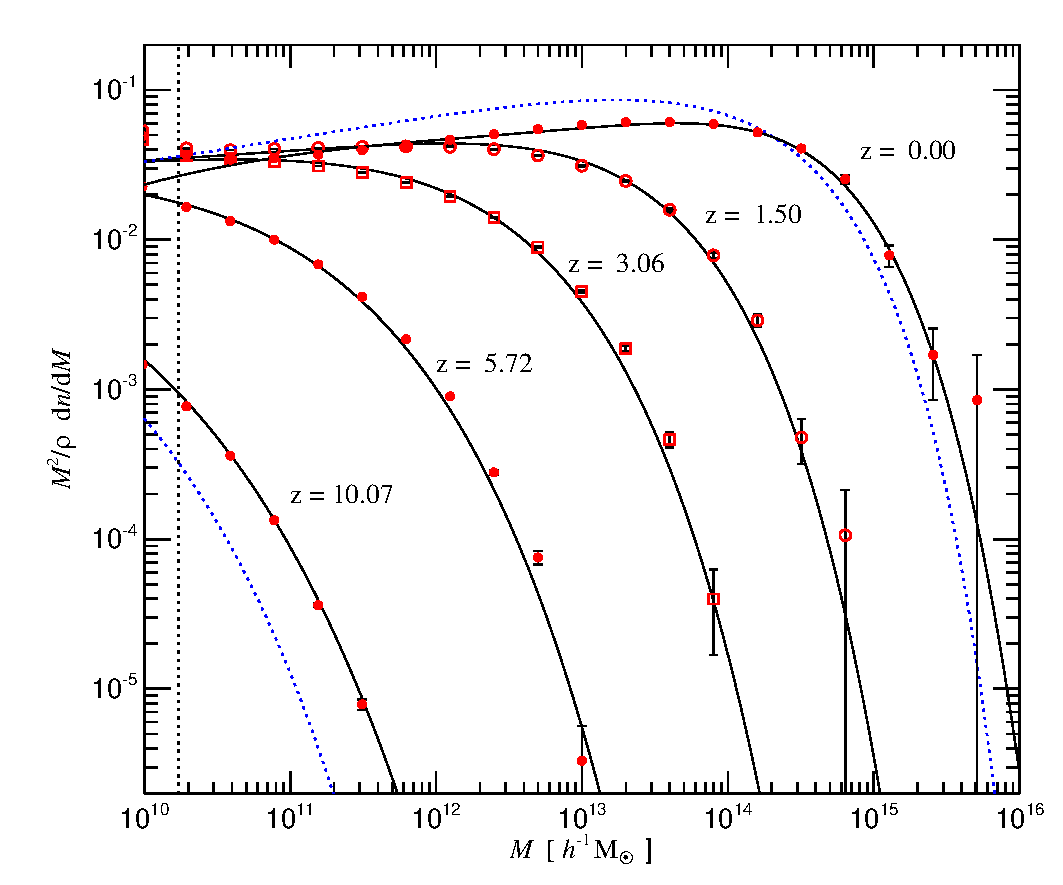
\includegraphics[scale=0.7]{Struct-halo_accretion.pdf}
%   \caption{A Millennium Simulation generated co-moving number density of 
%     dark matter halos, on the vertical axis, around which baryonic test
%     particles of high mass, on the horizontal axis, are gravitating. The
%     mass function of halos is given for different redshifts. The dotted
%     lines are the similar, analytic Press Schechter model. 
%   Credit: \cite{2005Natur.435..629S}}
%   \label{fig:Struct-halo_accretion}
%   \end{centering}
% \end{figure}
  
  The Millennium Simulation modeled the hierarchical evolution of large clouds 
  of CDM 
  interacting only though gravitation from a ``glasslike'' Gaussian 
  distribution just after decoupling to the current era and found that
  growth in the CDM filaments results in structures remarkably 
  similar to what is observed in the Universe today
  (\cite{desjacques2018large}). Fig. \ref{fig:Struct-power_spectrum} shows the 
  power spectrum of features in the density distribution that can be compared
  to observable redshifts
  (\cite{2005Natur.435..629S}). 

  \begin{figure}[H]
    \begin{centering}
    \includegraphics[scale=0.5]{Struct-power_spectrum.pdf}
    \caption{The dimensionless power spectrum at later redshifts of the
      Millennium Simulation model. Where \(\Delta^2\) approaches unity, 
      nonlinear growth takes over. Solid lines represent linear growth in the 
      Poisson distribution. The dashed line is the shot noise limit of the 
      model due to the number of bodies in the statistics.
    Credit: \cite{2005Natur.435..629S} Supplement}
    \label{fig:Struct-power_spectrum}
    \end{centering}
  \end{figure}

  % The correlation function of galaxies and galaxy clusters is not the same,
  % which indicates that neither is an unbiased tracer of matter density
  % fluctuations in general (\cite{desjacques2018large}).

% 6. Conclusions.
% Providing some concluding remarks and briefly comment on future tests of 
% the standard model.
\section*{Conclusions}
  $\Lambda$CDM explains much of the fossil evidence
  of the HBB origin, the features embedded in the CMB anisotropy 
  and the abundances of primordial elements in a universe that is 
  undergoing further nuclear processing. Dark matter and dark energy have an 
  unexplained origin in the current theory.

  Data from the Planck mission may indicate that universe has a closed 
  geometry after all, which challenges the inflation solution for the horizon
  and flatness problems (\cite{2020NatAs...4..196D}). Resolving the 
  curvature of spacetime is a fundamental test of the validity of 
  $\Lambda$CDM. 

  Further tests will attempt accounting for the dark sources of
  energy density in a way that satisfies the model. 


%  Primordial black holes are a potential MACHO candidate for dark matter, 
%  and may be a source of SNe Type 1a (\cite{PhysRevD.92.063007}), but their
%  existence may be exclusive of WIMPs (\cite{Adamek_2019}). 

% Constraining the free parameters of the physics of the Standard Model to
% fit the best observations of the universe today produces a benchmark model,
% which can be broken down into contributions of different 
% constituents to the energy density of the unverse in the following way,
% (\cite{ryden2003introduction}):

% \begin{center}
% \begin{tabular}{ c c c }
%   Photons & \(\Omega_{\gamma} = 5.35E-5 \) \\
%   Neutrinos & \(\Omega_{\nu} = 3.65E-5 \) \\
%   Total radiation & \(\Omega_{r} = 9.0E-5 \) \\
%   Baryonic matter & \(\Omega_{b} = 0.048 \) \\
%   Nonbaryonic matter & \(\Omega_{dm} = 0.262 \) \\
%   Total matter & \(\Omega_{m} = 0.31 \) \\
%   Cosmological constant & \(\Omega_{\Lambda} \approx 0.69 \)
%\end{tabular}
%\end{center}

%TC:ignore

\pagebreak
\begin{singlespace}
\printbibliography
\end{singlespace}

%TC:endignore

\end{document}

